\section{Обзор}
В главе выполнен обзор предметной области.
Описаны скрытые марковские модели и алгоритм Витерби,
а также приведены существующие решения, в которых этот 
алгоритм реализован для обработки большого объёма данных.
В заключительном разделе обзора рассмотрена техника специализации.

\subsection{Скрытые марковские модели}
\label{lab:HMM}
\emph{Скрытая марковская модель} (СММ)~\cite{Eddy_HMM}
является дискретным вероятностным автоматом, каждое состояние которого может с определённой вероятностью создавать наблюдение.
В определении СММ есть следующие параметры:
\begin{itemize}
	\item $\mathit{S_{1..N}}$ --- $N$ состояний автомата;
	\item $\mathit{O_{1..K}}$ --- $K$ возможных наблюдений;
	\item $\mathit{B_{1..N}}$ --- вероятности для каждого состояния из $\mathit{S_{1..N}}$ быть стартовым;
	\item $\mathit{T_{1..N, 1..N}}$ --- матрица переходов, $\mathit{T_{i,j}}$ является вероятностью перехода из состояния
$\mathit{S_{i}}$ в состояние $\mathit{S_{j}}$;
	\item $\mathit{E_{1..N, 1..K}}$ --- матрица наблюдений, 
где $\mathit{E_{i,j}}$ определяет вероятность создания наблюдения $\mathit{O_{j}}$ в состоянии $\mathit{S_{i}}$.
\end{itemize}
Пример скрытой марковской модели представлен на рисунке~\ref{fig:HMM}.
В ней два состояния H и L, и четыре возможных наблюдения A, C, T и G.
Вероятности переходов между состояниями указаны на соответствующих стрелках, а вероятности создания определённого наблюдения описаны в состояниях.

\begin{figure}
\centering
	\begin{subfigure}{\textwidth}
		\centering
		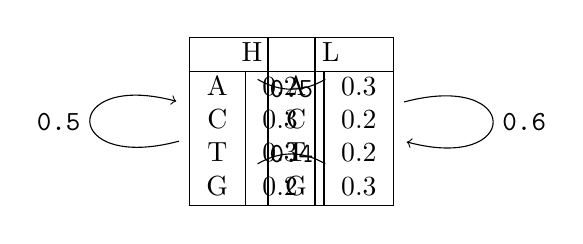
\begin{tikzpicture}
			\node (H) {
				\begin{tabular}{|c|c|}
					\hline
					\multicolumn{2}{|c|} H \\
					\hline
					A & 0.2 \\
					C & 0.3 \\
					T & 0.3 \\
					G & 0.2 \\
					\hline
				\end{tabular}
			};
			\node[right of=H] (L) {
				\begin{tabular}{|c|c|}
					\hline
					\multicolumn{2}{|c|} L \\
					\hline
					A & 0.3 \\
					C & 0.2 \\
					T & 0.2 \\
					G & 0.3 \\
					\hline
				\end{tabular}
			};
			\draw (H) edge[loop left] node {\tt 0.5} (H);
			\draw (H) edge[bend left] node {\tt 0.5} (L);
			\draw (L) edge[loop right] node {\tt 0.6} (L);
			\draw (L) edge[bend left] node {\tt 0.4} (H);
		\end{tikzpicture}
	\end{subfigure}
	\newline
	\vspace{1cm}
	\begin{subfigure}{\textwidth}
		\centering
		\begin{tabular}{c}
			Стартовые вероятности (B) \\
			\begin{tabular}{|c|c|}
				\hline
				H & L \\
				\hline
				0.5 & 0.5 \\
				\hline
			\end{tabular} \\
		\end{tabular}
		\vspace{0.3cm}
	\end{subfigure}
\caption{Пример СММ}
\label{fig:HMM}
\end{figure}


\subsection{Алгоритм Витерби}
\label{lab:Viterbi}
\emph{Алгоритм Витерби}~\cite{Viterbi} вычисляет для каждого состояния СММ (англ. HMM) максимальную вероятность нахождения в нём, при условии того, что последовательность событий \emph{Obs} была сгенерирована этой СММ.

\subsubsection{Описание методами динамического программирования}
\label{lab:dyn_Viterbi}
Алгоритм Витерби может быть описан методами динамического программирования.
Псевдокод алгоритма представлен на листинге~\ref{lab:dyn_Viterbi}.
Массивы индексируются с единицы до границы включительно.
На строках 5-6 происходит обработка первого наблюдения из последовательности $Obs$.
Так как это первое наблюдение, то вероятности перехода учитывать не нужно.
Вычисления, связанные с оставшейся частью последовательности, выполняются на строках 8-11.
Результатом является последняя строка матрицы $Dp$.
\begin{lstlisting}[caption=Алгоритм Витерби, label=Viterbi, escapeinside={(*}{*)}]
function Viterbi(HMM, Obs)
	lo = length(Obs)
	Dp[lo][HMM.N]

	for j = 1..HMM.N
		Dp[1][j] = HMM.E[j][Obs[1]] * HMM.B[j]
	
	for i = 2..lo
		for j = 1..N
			Dp[i][j] = 
					(*$\max_{x = 1..N}$*)(HMM.T[x][j] * HMM.E[j][Obs[i]] * Dp[i-1][x])

	return Dp[lo]
\end{lstlisting}


\subsubsection{Описание методами линейной алгебры}
\label{lab:LA_Viterbi}
Также алгоритм Витерби может быть выражен матричными 
операциями из линейной алгебры~\cite{LA_Viterbi}.
Рассмотрим подробнее, как это делается.

Ключевой идеей является использование специальной 
алгебраической структуры полукольцо \emph{Min-plus}.
Элементы полукольца будут описывать вероятности с
помощью вещественных чисел.
Операция сложения определяется как функция
минимума из двух чисел, а операция умножения имеет семантику
сложения чисел.
Нейтральными элементами по сложению будет $+\infty$ 
и 0 по умножению соответственно.
Ниже приведен пример умножения матрицы на столбец 
с использованием полукольца \emph{Min-plus}.
\[
  \begin{pmatrix}
    0 & 1 \\
    +\infty & 2
  \end{pmatrix}
  \begin{pmatrix}
    3 \\
    4
  \end{pmatrix}
  =
  \begin{pmatrix}
    min(0 + 3, 1 + 4) \\
    min(+\infty + 3, 2 + 4)
  \end{pmatrix}
  =
  \begin{pmatrix}
    3 \\
    6
  \end{pmatrix}
\]

Для того, чтобы можно было использовать полукольцо \emph{Min-plus}, 
ко всем вероятностям $p$ в СММ применяется 
преобразование~\ref{eq:t}.
Это делается для сохранения точности расчетов.
Далее такая вероятность будет называться \emph{преобразованной}.
Например, преобразованная вероятность 0.5
равна $-1 * log_2(0.5) = 1$.
\begin{equation}
t(p) =
	\begin{cases}
	p > 0: & -1 * log_{2}(p))\\
	p = 0: & +\infty
	\end{cases}       
  \label{eq:t}
\end{equation}

Для каждого события \emph{o} из множества \emph{O} 
определяем диагональную матрицу $P(o)$ размера $N \times N$.
\[
  P(o) =
  \begin{pmatrix}
    t(E[1,o]) & \hdots & +\infty \\
    \vdots & \ddots & \vdots\\
    +\infty & \hdots & t(E[N,o])
  \end{pmatrix}
\]

Начало алгоритма Витерби --- это обработка первого наблюдения 
из последовательности \emph{Obs}.
В столбце \emph{B} хранятся преобразованные вероятности 
состояний из СММ быть начальными.
Символ $\times$ обозначает умножение матриц с использованием 
полукольца \emph{Min-plus}:
\[Probs_{1} = P(Obs[1]) \times B.\]
Далее вычисляются преобразованные вероятности для всех 
состояний СММ с учётом ос\-тавшихся событий из \emph{Obs}.
Матрица \emph{T} хранит преобразованные вероятности 
переходов из состояния в состояние.
В отличие от обработки первого наблюдения, далее необходимо 
учитывать и вероятности перехода, и вероятности создания 
наблюдения.
Обработка происходит следующим образом:
\[Probs_{t} = P(Obs[t]) \times T^{\top} \times Probs_{t - 1}.\]
После выполнения всех шагов алгоритма, в столбце 
\emph{Probs\textsubscript{lo}}, где $lo$ --- это длина 
последовательности $Obs$, будут находиться преобразованные 
вероятности быть в определённом состоянии СММ при условии 
наблюдения последовательности событий \emph{Obs}.
Псевдокод алгоритма приведен на листинге~\ref{LA_Viterbi}.
\begin{lstlisting}[caption={Алгоритм Витерби, выраженный методами линейной алгебры}, label=LA_Viterbi, escapeinside={(*}{*)}]
function Viterbi(HMM, Obs)
	lo = length(Obs)
	// (*\textcolor{codegreen}{Столбец для результатов}*)
	Probs[1][HMM.N]

	// (*\textcolor{codegreen}{Все матричные умножения выполняются в полукольце Min-plus}*)
	Probs = P(Obs[1]) (*$\times$*) HMM.B
	
	for i = 2..lo
		Probs = P(Obs[i]) (*$\times$*) (HMM.T)(*$^{\top}$*) (*$\times$*) Probs
		
	return Probs
\end{lstlisting}


\subsection{Существующие реализации алгоритма Витерби}
\label{lab:exist_Viterbi}
В данном разделе рассмотрены существующие 
высокопроизводительные реализации алгоритма Витерби, которые 
используются на практике в бионформатике для решения задачи 
гомологичности, то есть для определения схожести протеинов.
Группы схожих протеинов называются \emph{семейством},
на основе которого можно построить СММ, описывающую общие 
части протеинов из семейства.
Такая СММ называется \emph{профилем}.
Все протеины кодируются двадцатью аминокислотами, 
которые могут быть выражены буквами латинского алфавита.
Последовательность, обрабатываемая с помощью профиля, также 
является закодированным протеином.

Рассмотренные далее реализации алгоритма Витерби выполнены с 
использованием метода динамического программирования.
Этот метод описан в подразделе~\ref{lab:dyn_Viterbi}.

\subsubsection{\name{HMMer}}
\label{lab:HMMer}
Решение \name{HMMer}~\cite{HMMer} используется для поиска в базах 
данных последовательностей гомологов исследуемых протеинов, а 
также для создания профилей семейств протеинов.
Этот проект является открытым (open source project), реализован  на языке C с возможностью
использовать SIMD-инструкции процессора.
Успешно применяется во многих базах данных, таких как \name{Pfam}~\cite{Pfam}.

Авторами проекта были предложены вероятностные \emph{фильтры}.
Их применение позволяет ускорить обработку данных из-за 
уменьшения вычислений в алгоритме Витерби за счет уменьшения 
количества состояний и переходов в СММ.
Один из таких фильтров --- \name{MSV} (Multiple Segment 
Viterbi)~\cite{MSV_Eddy}.

\subsubsection{\name{CUDAMPF}}
\label{lab:CUDAMPF}
В проекте \name{CUDAMPF}~\cite{cudampf} реализованы
вероятностные фильтры из существующего решения \name{HMMer} с использованием 
\name{CUDA}.
Код предназначен для видеокарт \name{NVIDIA} с 
архитектурой \name{Kepler} или более новой.
Проект рассчитан на определение гомологичности одновременно 
для множества протеинов.

Авторы предлагают четыре уровня параллелизма.
Первые три основаны на логическом параллелизме по данным.
Четвертый уровень использует \name{SIMD}-инструкции 
вычислителей видеокарты.
Разделение данных по уровням позволило добиться ускорения в 
23,1 раз при работе с фильтром \name{MSV} по сравнению с
\name{HMMer}.

Несмотря на то, что авторами заявлена корректность 
реализации, в исходном коде есть гонка данных при вычислении 
одного из состояний при обработке \name{MSV}.
В этом состоянии хранится максимум из определённого множества состояний.
В коде \name{CUDAMPF} переменная, хранящая максимум, 
не защищена от одновременной записи двумя или более потоками.

\subsection{Специализация}
Техника \emph{специализации} (или \emph{частичных вычислений}) предназначена для
преобразования программ, у которых часть входных параметров
известна и зафиксирована~\cite{Jones_spec} с целью оптимизации производительности.
Типичным случаем для специализации является последовательное 
применение программы для обработки данных, часть из которых 
не меняется от запуска к запуску.
Согласно определениям, которые приняты для специализации, 
зафиксированные параметры называются \emph{статическими}, а 
все остальные параметры --- \emph{динамическими}.
Цель применения специализации --- уменьшить количество 
вычислений, которые зависят от статических параметров.
Ожидается, что при многочисленных запусках специализированная 
программа на динамических параметрах будет более 
производительной чем изначальная версия программы, которая 
выполняется на статических и динамических параметрах.
Распространённой проблемой на практике является замедление 
производительности из-за большого объема специализированного
кода.
Схема специализации приведена на рисунке~\ref{spec}.
\begin{figure}[h!]
  \centering
  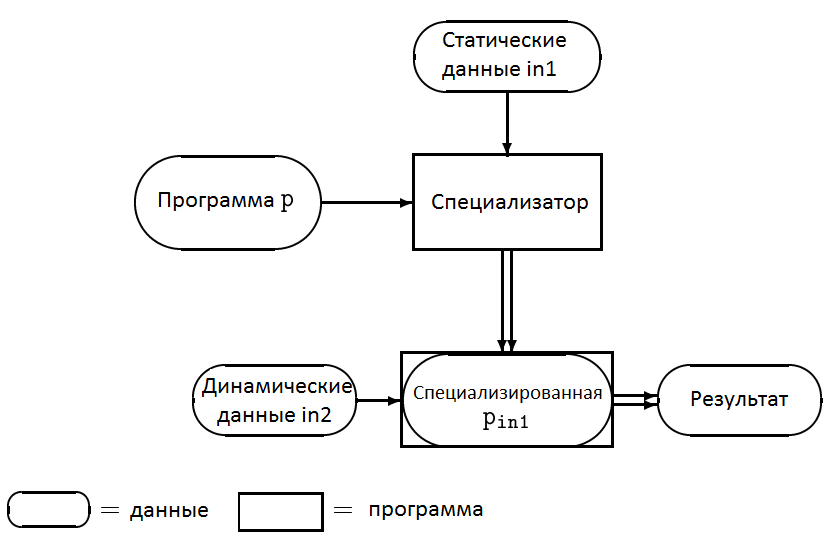
\includegraphics[width=\columnwidth]{spec.png}
  \caption{Концептуальная схема специализации\protect\footnotemark}
  \label{spec}
\end{figure}
\footnotetext{Схема взята из книги~\cite{Jones_spec}, и содержание схемы переведено на русский язык.}

Специализация была успешно применена в обработке 
графики~\cite{RT_spec}, обработке запросов к базам 
данных~\cite{SQL_spec} и поиску подстроки в строке на 
GPGPU~\cite{part_eval_GPU}.
Более подробно о специализации можно узнать в книге Джонса, 
Гомарда и Сестофта \cite{Jones_spec}.

Специализация может применяться как и к произвольным 
программам, так и к отдельным реализациям какого-то 
алгоритма.
Независимо от того, что специализируется, создание 
оптимального специализатора является алгоритмически 
неразрешимым, это можно доказать через сведение к проблеме 
останова.
В случае специализации какого-то заранее выбранного 
алгоритма, можно использовать его шаги и структуру для 
создания более эффективной специализированной версии.
Далее будет рассмотрен алгоритм создания специализированной 
версии алгоритма Витерби.
